%% Supporting Information for the ITOR manuscript. Generated by code/build_itor_si.py
%% from paper/routing_model_orf.tex; do not edit by hand.
\documentclass[11pt,letterpaper]{article}
\usepackage[margin=1in]{geometry}
\usepackage{mathptmx}
\usepackage{setspace}
\setstretch{1.1}
\usepackage{amsmath,amssymb,booktabs,array,graphicx,microtype,float}
\usepackage{xcolor}
\usepackage{caption}
\captionsetup{labelfont=bf,labelsep=period,font=small}
\usepackage[authoryear,round]{natbib}
\let\cite\citep
\usepackage{hyperref}
\hypersetup{colorlinks=true,linkcolor={blue!55!black},citecolor={blue!55!black},urlcolor={blue!55!black}}
\providecommand{\bibcommenthead}{}
\setlength{\emergencystretch}{3em}
\usepackage{tocloft}
\setlength{\cftsecnumwidth}{2.4em}
\setlength{\cftsubsecnumwidth}{3.6em}
\makeatletter
\def\input@path{{../paper/}}
\makeatother
\graphicspath{{../paper/}}
\renewcommand{\thesection}{S\arabic{section}}
\renewcommand{\thetable}{S\arabic{table}}
\renewcommand{\thefigure}{S\arabic{figure}}
\renewcommand{\theequation}{S\arabic{equation}}
\input{result_macros_v7.tex}
\input{result_macros_v8.tex}
\input{result_macros_v9.tex}
\input{result_macros_v10.tex}
\input{result_macros_v11.tex}
\input{result_macros_v12.tex}
\title{Supporting Information for ``Reliability screening for vehicle routing with
time windows: a solver-independent alternative to travel-time padding''}
\author{Suhan Ali}
\date{}
\begin{document}
% same order of the four Ali (2026) records as in the main text, so their letters a--d match
\nocite{ali2026freeze,ali2026freeze2,ali2026freeze3,ali2026archive}
\maketitle
\noindent This document gives the full model, the design of every study, every result table and the
further exploratory checks. All numbers are generated from the records in the archive
\citep{ali2026archive}.
\tableofcontents
\clearpage
\section{Problem definition}\label{sec:si-model}

Let $N=\{0,1,\ldots,n\}$ be the nodes, with depot 0 and customers
$C=N\setminus\{0\}$. Let $V$ be a homogeneous fleet. Customer $i$ has demand
$\delta_i$, deterministic service time $s_i$, and offered service-start window
$[l_i,u_i]$. Vehicle capacity is $Q$, and the maximum shift duration is
$H^{\max}$. The nominal distance and planning time on arc $(i,j)$ are $d_{ij}$
and $\bar t_{ij}$.

The planning variables are $x_{ijv}\in\{0,1\}$ for arc use,
$z_{iv}\in\{0,1\}$ for customer assignment, $y_v\in\{0,1\}$ for vehicle use,
service-start time $a_{iv}$, depot departure $d_v$, depot return $r_v$, and
slack deficit $G_{iv}\geq0$. The assignment variables give each customer one
vehicle and activate the corresponding customer--vehicle copy:
\begin{align}
 \sum_{v\in V} z_{iv} &= 1 && i\in C, \\
 \sum_{j\in N\setminus\{i\}}x_{ijv}
   =\sum_{j\in N\setminus\{i\}}x_{jiv} &= z_{iv}
      && i\in C,\ v\in V, \\
 \sum_{j\in C}x_{0jv}=\sum_{i\in C}x_{i0v} &= y_v
      && v\in V.                                            \label{eq:flow}
\end{align}
Because demand is delivery-only, route capacity needs no cumulative-load
variables:
\begin{equation}
 \sum_{i\in C}\delta_i z_{iv}\leq Qy_v \qquad v\in V.       \label{eq:capacity}
\end{equation}
The time-propagation constraints below rule out customer-only subtours: summing
them around any directed customer cycle would give
$0\geq\sum_i(s_i+\bar t_{ij})>0$. The argument does not need positive demands.
Time windows apply only to assigned copies:
\begin{equation}
 l_i z_{iv}\leq a_{iv}\leq u_i z_{iv}
 \qquad i\in C,\ v\in V.                                   \label{eq:activate}
\end{equation}
Separate departure and return variables avoid using one time variable for two
depot visits. With a valid global deactivation constant
$M\geq H^{\max}+\max_i s_i+\max_{ij}\bar t_{ij}$,
\begin{align}
 a_{jv} &\geq d_v+\bar t_{0j}-M(1-x_{0jv}), \\
 a_{jv} &\geq a_{iv}+s_i+\bar t_{ij}-M(1-x_{ijv}), \\
 r_v &\geq a_{iv}+s_i+\bar t_{i0}-M(1-x_{i0v}).              \label{eq:time}
\end{align}
The bounds $0\leq d_v,r_v\leq H^{\max}y_v$ deactivate unused vehicles, and
$r_v-d_v\leq H^{\max}y_v$. The code enforces these timing relations through
OR-Tools routing dimensions and never builds these time constraints explicitly, so no
big-$M$ relaxation or big-$M$ diagnostic is claimed for the code.

For target slack $s^*$,
\begin{align}
 G_{iv} &\geq a_{iv}-(u_i-s^*)z_{iv}, \\
 G_{iv} &\geq 0.                                            \label{eq:slack}
\end{align}
At the optimum, $G_{iv}=\max\{0,s^*-(u_i-a_{iv})\}$ when $z_{iv}=1$, and
$G_{iv}=0$ when the customer is not assigned to vehicle $v$.

\section{Candidate objectives and scaling}\label{sec:objective-scaling}

The four raw criteria are
\begin{align}
 F_1 &= c_f\sum_{v\in V}\sum_{i,j\in N}d_{ij}x_{ijv},
 &F_2 &= \sum_{v\in V}\sum_{i\in C}G_{iv},\\
 F_3 &= \sum_{v\in V}(r_v-d_v),
 &F_4 &= \sum_{v\in V}y_v.                                 \label{eq:criteria}
\end{align}
$F_3$ counts driving, service and waiting time, and each vehicle may
leave the depot when it suits the schedule, so no vehicle is charged for waiting
at the depot before its first service can start.

Reference values come from four heuristic solves, each minimizing one criterion.
For each criterion $k$, $L_k$ and $U_k$ are the smallest and largest values
among these anchor solutions. They are \emph{scaling ranges}, not utopia and
nadir points, and need not bound the Pareto frontier. No value is clipped. The
normalized score is
\begin{equation}
 Z(\mathbf{x})=\sum_{k=1}^{4}w_k\frac{F_k(\mathbf{x})-L_k}{\max\{U_k-L_k,1\}}. \label{eq:objective}
\end{equation}
The floor of 1 in the denominator avoids division by zero when a discrete
criterion takes the same value in every anchor solution. The baseline weights
$\mathbf{w}=(0.5693,0.2643,0.1055,0.0609)$ are a fixed experimental preference
vector that defines the candidate-selection objective. They were fixed before any
experiment reported here, were not elicited from a fleet operator, and make no
claim about the preferences of any industry. No result relies on how they were
first obtained. For completeness, Section~\ref{sec:ahp-matrix} and
\texttt{code/ahp\_weights.py} record their origin: the principal eigenvector of
an Analytic Hierarchy Process matrix \cite{saaty1980} set for an earlier list of
criteria, whose third criterion, total distance, later became driver duration
without the matrix being revised. Section~\ref{sec:weights} varies the weights
directly. The weights shape the candidates
and rank the admitted ones, but the admission test and the validation do not use
them. Any scalar objective could take the place of $Z$ without changing how
reliability is judged; the robust comparison (Section~\ref{sec:robust-design})
uses distance alone. The results do depend on the objective: with equal weights
the advantage over conservative speed fell by more than half
(Section~\ref{sec:weights}).

In OR-Tools, distance is an arc cost, driver duration is a span cost on each
vehicle's time dimension, slack deficit is a soft upper bound at each customer,
and fleet use is a fixed cost per vehicle. Integer coefficients are scaled once
per criterion. The main planning matrix is nominal and fixed, so the original
candidate generator does not use clock-dependent travel times. The
\emph{conservative-speed} baseline replaces 40 km/h with 33.3 km/h throughout the
planning matrix. This pads every trip by 20\%, including off-peak trips, so the
comparison does not isolate the value of knowing when the peak occurs.

\subsection{Clock-aware approximation and deterministic guarantee}

A separate distance heuristic uses the time of day. For each origin, it freezes
the departure time estimated from the previous schedule, integrates
\eqref{eq:fifo} at that time to build the origin's outgoing travel-time row, and
solves again. Two passes receive 2.5 seconds each. The first reference schedule is
the retained nominal plan, whose solve cost has already been incurred
separately. For a customer, the
departure estimate is the service start plus the service time. For a depot arc,
it is the previous departure for the first customer of each route and the mean of
the used depot departures for other customers. Each resulting route sequence is
rescheduled with the exact deterministic FIFO profile, and binary search finds its
latest feasible whole-minute depot departure. Routes that fail even when leaving
at time zero are rejected. The shortest deterministically feasible output is
kept, with duration breaking ties. The method is an approximation that reports
its failures; it is not a departure-dependent callback or an exact optimizer for
the time-dependent VRPTW.

For a feasible conservative-speed plan, the evaluation speed at $\sigma=0$ never
drops below the planning speed during the planned shift. Starting from the same
depot departure, FIFO and induction along each route show that the evaluated
service starts and the return happen no later than planned. At $\sigma=0$, such
a plan serves every customer on time by construction. The deterministic
feasibility of the clock-aware approximation is also checked before a plan is
accepted. Neither property is an experimental reliability gain.

\section{Time-dependent stochastic evaluation}

\subsection{FIFO travel times}

Partition the day into periods $[T_k,T_{k+1})$ with strictly positive speeds
$\nu_k$. The deterministic time-dependent travel time $t_{ij}(\tau)$ is the
smallest $\Delta\geq0$ satisfying
\begin{equation}
 \int_{\tau}^{\tau+\Delta}\nu(u)\,du=d_{ij},
 \qquad \nu(u)=\nu_k\text{ for }u\in[T_k,T_{k+1}).           \label{eq:fifo}
\end{equation}
Because the distance covered grows strictly with time, the arrival map
$\tau\mapsto\tau+t_{ij}(\tau)$ is nondecreasing, so FIFO holds.

\subsection{Correlated disturbances}

For scenario $\omega$, arc travel is
\begin{equation}
 T_{ij}(\tau,\omega)=t_{ij}(\tau)\Omega_{ij}(\omega),
\end{equation}
where
\begin{align}
 \Omega_{ij}(\omega)&=\exp\{\varepsilon_{ij}(\omega)\},\\
 \varepsilon_{ij}(\omega)&=\sigma\left(
 \sqrt{\rho}\,\xi_0(\omega)+\sqrt{1-\rho}\,\xi_{ij}(\omega)\right).
                                                               \label{eq:noise}
\end{align}
Here $\rho$ is the correlation between the latent Gaussian log-errors. It is
not the Pearson correlation between the multipliers, which is
\begin{equation}
 \operatorname{Corr}(\Omega_i,\Omega_j)
 =\frac{\exp(\sigma^2\rho)-1}{\exp(\sigma^2)-1}.
\end{equation}
The multiplier has median 1 and mean $\exp(\sigma^2/2)$, so the deterministic
profile gives the median travel time, which is slightly below the mean.

Scenario banks do not depend on the order in which routes are evaluated. A common
factor is drawn once per scenario, and each directed arc gets its own
pseudorandom stream keyed by the bank seed and the arc's endpoints. Plans
evaluated on the same bank see identical disturbances on the arcs they
share.

\section{Screening and independent validation}

For a fixed plan $R$ and scenario $\omega$, let
\begin{equation}
 q(R,\omega)=\frac{1}{|C|}\sum_{i\in C}
 \mathbf{1}\{a_i(R,\omega)\leq u_i\}
\end{equation}
be the on-time customer proportion. The primary service event is
\begin{equation}
 J_{\kappa}(R,\omega)=\mathbf{1}\{q(R,\omega)\geq\kappa\},
 \qquad \kappa=0.95,                                        \label{eq:event}
\end{equation}
and the target is
\begin{equation}
 \Pr[J_{\kappa}(R,\omega)=1]\geq\alpha,
 \qquad \alpha=0.95.                                       \label{eq:chance}
\end{equation}
The stricter probability that no customer in the fleet is late on a given day
is also reported. It is not used for admission, because it falls mechanically as
the number of customers grows.

For $N$ scenarios and empirical success $\hat p$, the one-sided Wilson lower
bound at confidence $1-\eta$ is
\begin{equation}
 L(\hat p)=
 \frac{\hat p+z^2/(2N)-z\sqrt{\hat p(1-\hat p)/N+z^2/(4N^2)}}
 {1+z^2/N},\qquad z=z_{1-\eta}.                             \label{eq:wilson}
\end{equation}

Candidate generation contracts only the internal planning deadline, to
$[l_i,\max\{l_i,u_i-\beta\}]$. The offered window $[l_i,u_i]$ does not change,
and every scenario is scored against the original $u_i$. For each buffer
$\beta$, a candidate is generated with the slack-aware objective and assessed on
the screening bank. The anchor ranges come from the uncontracted ($\beta=0$)
instance and stay fixed across the buffer search. Among the candidates whose
screening lower bound reaches $\alpha$, the one with the smallest normalized
planned score \eqref{eq:objective} is selected. In simulation every vehicle
leaves at its planned $d_v$; departure times do not change with the scenario.
The selected plan is then evaluated once on a larger, untouched validation bank,
so the search never selects on the evidence used for the final report. The
lower bound holds for each candidate separately, while the search covers 13
buffer levels; Section~\ref{sec:familywise} repeats the selection with a
Bonferroni bound over the grid.

A prespecified fallback makes the procedure's output defined on every instance.
If no candidate passes screening, the procedure returns the uncontracted
slack-aware plan ($\beta=0$). Validation never changes this choice; it only
estimates the performance of the plan already chosen. Results for selected plans alone are always labelled as such, and
the main procedure comparison includes all instances.

Three reliability quantities appear in the results, and each answers a different
question:
\begin{itemize}
  \item[$\bullet$] \textbf{Admission criterion.} The Wilson lower bound \eqref{eq:wilson} on
        the screening bank, computed for each candidate. A candidate is admitted
        when it reaches $\alpha=0.95$.
  \item[$\bullet$] \textbf{Selected-plan probability.} The validated estimate of
        $\Pr[J_\kappa=1]$ for a plan that passed screening, from the untouched
        bank.
  \item[$\bullet$] \textbf{Procedure-level probability.} The validated probability averaged
        over all instances, including those on which screening admitted nothing
        and the fallback was returned.
\end{itemize}
The chance constraint \eqref{eq:chance} is what screening tests for each
admitted plan. The procedure-level average falls below $\alpha$ whenever fallback
plans are weaker, so the results report admitted plans and the whole procedure
separately. The 95\% target is the admission standard for each plan, tested
with a per-candidate 95\% lower bound. It applies to admitted plans only; where
nothing is admitted, the procedure returns the fallback, which has not passed
this test.

\subsection{Screened conservative speed and reachability-capped contraction}\label{sec:capping}

Screened conservative speed uses the same buffer grid, admission bank and
Wilson threshold, but its candidates minimize distance on the padded matrix.
Among the passing plans it chooses the shortest, breaking ties by planned
duration and then by buffer. Its fallback is the uncontracted conservative plan,
or the retained uncontracted slack-aware plan if no conservative plan was found.
The procedure's output is therefore defined on all 53 instances, while the
conservative generator itself still finds a plan on 46 of them.

Let $e_i=\max\{l_i,\bar t_{0i}\}$ be the earliest direct service time under the
nominal matrix. The capped weighted variant uses the internal upper bound
\begin{equation}
 u_i^{\rm cap}(\beta)=\min\{u_i,\max\{l_i,u_i-\beta,e_i\}\}.
\end{equation}
This stops contraction alone from making a customer unreachable by a direct
trip when it was reachable before. It does not guarantee that a joint routing is
feasible or that the admission target is met. When a contracted model is
identical to one already solved, its archived candidate is reused; only changed
models are solved again. Selection still uses the fixed original scaling ranges,
the weighted score and the same fallback.

To diagnose failures, a shortest-path relaxation uses arc cost
$\bar t_{ij}+s_i$ (with $s_0=0$) and allows intermediate customers without
capacity or window restrictions. Its depot-to-$i$ distance is a valid lower bound
even if rounded distances violate the triangle inequality. A contracted deadline
below this bound certifies infeasibility. When there is no certificate, a missing
solver output is labelled \emph{no feasible plan found}: reaching the time limit
without a plan does not prove infeasibility, and passing the reachability test
does not prove feasibility. Solver status information was not
kept in the archived runs and is not inferred afterwards.

\section{Experimental design}

Synthetic instances place a central depot and uniformly distributed customers
on a $100\times100$ grid. Demand is uniform on 10--49 units, service time is
10 minutes, window width is uniform on 90--149 minutes, capacity is 1000, and
the shift limit is 600 minutes. Time zero is 06:00 local time, so clock time is
the relative schedule time plus 360 minutes. Table~\ref{tab:design} gives the
seeded instance sizes, and Table~\ref{tab:parameters} lists every model and
simulation constant.

\begin{table}[ht]
\centering
\caption{Seeded synthetic experimental design.}
\label{tab:design}
\begin{tabular}{rrrr}
\toprule
Customers & Vehicles available & Instances & Seeds\\
\midrule
20  & 6  & 20 & 7200--7219\\
50  & 14 & 15 & 7500--7514\\
100 & 26 & 10 & 8000--8009\\
200 & 40 & 8  & 9000--9007\\
\bottomrule
\end{tabular}
\end{table}

\begin{table}[ht]
\centering
\small
\caption{Planning, disturbance, and statistical parameters.}
\label{tab:parameters}
\begin{tabular}{p{0.42\textwidth}p{0.46\textwidth}}
\toprule
Parameter & Value \\
\midrule
Nominal/free-flow speed $\bar v$ & 40 km/h \\
Shift and clock origin & 600 min, beginning 06:00 local time \\
Capacity; service time; target slack $s^*$ & 1000; 10 min; 15 min \\
Distance cost $c_f$ & 15 cost units/km \\
Objective weights $(w_1,w_2,w_3,w_4)$ & $(0.5693,0.2643,0.1055,0.0609)$ \\
Integer objective scale & 100,000 \\
Planned-shift speed divisors &
$0.9$ (06:00--07:00), $1.2$ (07:00--09:00), and $1.0$
(09:00--16:00); speed is $\bar v$ divided by the divisor \\
Outside-shift continuation & 1.0 to 17:00, 1.3 (17:00--19:00), 0.9 thereafter;
used if a stochastic route overruns the shift \\
Log-error scale $\sigma$; latent correlation $\rho$ & 0.20; 0.50 \\
Exploratory disturbance grid & $\sigma\in\{0.10,0.20,0.30\}$;
$\rho\in\{0,0.5,0.9\}$ \\
Service fraction $\kappa$; target $\alpha$ & 0.95; 0.95 \\
Wilson tail probability $\eta$ & 0.05 (one-sided 95\% lower bound) \\
Screening; validation; sensitivity scenarios & 1000; 5000; 1000 per cell \\
Buffer grid & $\beta\in\{0,5,\ldots,60\}$ min \\
\bottomrule
\end{tabular}
\end{table}

Eight configurations are compared in the development study:
\begin{enumerate}
  \item \textbf{Nominal distance}: fixed 40 km/h planning matrix and a
        distance-minimizing objective.
  \item \textbf{Conservative-speed distance}: distance minimization with a
        uniform 33.3 km/h planning matrix.
  \item \textbf{Slack-aware}: objective \eqref{eq:objective} with $\beta=0$,
        which shows the effect of the objective without screening.
  \item \textbf{Fleet-matched distance}: distance minimization forced to use
        exactly as many vehicles as the slack-aware plan, starting from its
        feasible routes.
  \item \textbf{Original procedure}: the complete weighted internal-buffer search, with
        selection on 1000 screening scenarios, the prespecified $\beta=0$
        fallback, and assessment on 5000 fresh scenarios.
  \item \textbf{Screened conservative}: conservative-speed distance candidates
        with the same admission test and the fallback defined above.
  \item \textbf{Capped procedure}: the original weighted procedure with
        customer-specific reachability caps.
  \item \textbf{Clock approximation}: two matrix updates from estimated
        departure times, followed by exact deterministic rescheduling.
\end{enumerate}

The nominal shift ends at 16:00. The full-day speed profile continues past
that time, because lognormal delays are unbounded and a stochastic route can
overrun. Evening periods lie outside the planned shift but stay in the evaluator.
Fleet-matched distance starts from the slack-aware routes. Because this could
carry over their structure, the starting point is treated as part of that
comparator's definition.

The screening grid is $\beta\in\{0,5,\ldots,60\}$ minutes. The four
single-criterion anchor solves get two seconds each to stabilize the scaling
ranges, and each candidate solve gets a five-second OR-Tools budget. If a
candidate solve returns no feasible plan, the same five-second call is repeated
at most twice more. The first feasible result is kept; there is no best-of-several
selection. A new model with a reachability certificate is not solved at all. The
clock approximation splits one five-second budget between its two solves. Six
experiment workers ran in parallel, and elapsed times and software versions are
recorded. Within an instance, every configuration uses the same fresh validation
bank.

The reliability outcomes are service-event probability, zero-lateness fleet-day
probability, mean on-time fraction, expected number of late customers, mean and
95th-percentile total lateness, and mean route success. The operational outcomes
are distance, driver duration and fleet use. Simulated duration under the common
evaluation model is also reported, to separate actual route time from each
generator's planned $F_3$. Differences are paired by instance, and intervals
across instances are kept separate from binomial Monte Carlo intervals within an
instance. Across-instance intervals use a paired nonparametric bootstrap with
20,000 resamples and a fixed analysis seed. A claim that distances are equivalent
would need a prespecified equivalence margin, so failing to reject a difference
is not treated as proof of equality.

\section{First confirmatory study and weight-sensitivity design}\label{sec:confdesign}

A confirmatory protocol was fixed before any new instance was generated or
solved. It sets out four directional hypotheses, their tests and decision rules,
a failure policy, and 53 instance seeds equal to the development seeds shifted by
60000. The protocol, the code that runs and analyses it, and a SHA-256 manifest
of those files were committed to a public repository (commit
\texttt{41fae67d\allowbreak 9520bd5d\allowbreak d01fcac8\allowbreak 7e680a5a\allowbreak 69325d10}) and archived on Zenodo
\cite{ali2026freeze} before the study was run. The analysis program will not run
unless the complete prescribed study is present and every frozen file matches
the manifest.

Each hypothesis concerns validated service-event probability on the fresh bank,
with the instance as the unit. H1 (primary): on instances where
conservative-speed planning returns a plan, the original procedure exceeds it.
H2 (primary): on all instances, the capped procedure exceeds the original
procedure. H3: screening admits the capped procedure on more instances than the
original procedure, tested with an exact McNemar test at the 0.05 level. H4: on
the instances of H1, the advantage of the original procedure over conservative
speed is larger at $\sigma=0.30$ than at $\sigma=0.10$ with $\rho=0$. H1 and H2
use 97.5\% intervals, a Bonferroni adjustment for two primary hypotheses, and
each is confirmed only if its paired bootstrap interval lies above zero. H4 uses
a 95\% interval. H3 and H4 are secondary: they carry less weight than H1 and H2
and cannot rescue an unconfirmed primary hypothesis. Holm's procedure in place
of the Bonferroni adjustment would not change either primary decision. H4
compares fixed plans: each plan is screened under the primary setting
($\sigma=0.20$, $\rho=0.5$) and then evaluated across the sweep without
re-screening. In this paper, a hypothesis is \emph{confirmed} when it meets the
decision criterion fixed in its protocol, and nothing more is meant. All three
protocols are confirmatory only within the prespecified synthetic setting: their
instances come from the generator and disturbance model of the development
study, so they test repeatability there and are not external validation. H2
and H3 both measure the effect of capping, one on service and one on admission,
so they are two views of one change.

A configuration without a plan scores zero on that instance, in validation and
in every sweep cell, so a failure counts against the configuration that failed.
A software error is recorded with its traceback, is never scored as routing
performance, and blocks the analysis.

Parameters, budgets and scenario counts are those of the development study
(Table~\ref{tab:parameters}). The study ran on an Apple M1 Pro laptop with ten
cores under macOS 26.3.1, with Python 3.12.15, NumPy 2.5.3 and OR-Tools
9.15.6755; the development runs used Python 3.12.14 on Linux. Stage 1 ran the
four instance sizes as four parallel processes, where the written protocol lists
a sequential loop, and stage 2 used six workers as specified. These are the
deviations from the written procedure. The scheduling change affects only the CPU
time available to each time-limited solve.

The weight analysis is exploratory. The original procedure was rerun on the
development instances with four weight vectors: the original vector, the original
with its two largest weights swapped, a distance-heavy vector and equal weights
(Section~\ref{sec:weights}). Each rerun regenerates the candidate family,
screens it on the same bank and validates the selected plan or fallback on the
same fresh bank, with the same five-second budget. The vectors were chosen before
the runs, and each was run once; a later bracketing run, also exploratory,
repeated the original and equal vectors and added two more
(Section~\ref{sec:weights}).

The benchmark check is also exploratory. It uses the eight R1 and RC1 Solomon
files available in the ML4VRP 2024 competition repository \cite{ml4vrp2024},
which hosts Solomon's instances \cite{solomon1987}. The C1 instances are left out
because their horizon of 1236 time units is longer than one working shift.
Coordinates are read as kilometres, with the study's rounded Euclidean distances
and a planning speed of 40~km/h, so one Solomon time unit equals 1.5 minutes.
Ready and due times are multiplied by 1.5 and rounded down, service time becomes
15 minutes, and the capacity of 200 and the 25 vehicles are kept. The shift
length is the scaled depot due time, 345 minutes for R1 and 360 minutes for RC1,
and the shift starts at 06:00 so that the morning peak falls inside it. Planning
times are rounded up to whole minutes, as in the main study. This mapping keeps
Solomon's relation between travel time and window width, because one distance
unit takes one Solomon time unit to drive at the planning speed. The C1 instances
could be fitted by compressing time, but that would change how tight their
windows are relative to travel times, so the eight instances are a convenience
sample of the R1 and RC1 types. The pipeline code is unchanged; only the instance
loader and the parameter constructor are replaced.

\section{Second confirmatory study design}\label{sec:conf2design}

The first confirmatory study left two questions open. Its candidate generator
produces weaker routes than the state of the art, so the benefit of screening
might shrink with candidates from a stronger search. Its post hoc analysis also
suggested that returning the conservative-speed plan when screening admits
nothing would raise pooled service (Section~\ref{sec:confirmatory}), but that
rule was chosen after the results were seen. A second protocol tested both
questions on 53 further instances, with seeds equal to the development seeds
shifted by 80000.

The second generator is the hybrid genetic search of PyVRP
\cite{vidal2022,wouda2024}, version 0.14.0. It solves the same planning model as
the OR-Tools generator: the static matrix at the planning speed, hard and possibly
contracted windows, capacity, shift length and fleet size, with each vehicle
leaving at the latest feasible time. Its weighted objective keeps the distance,
driver-duration and fleet terms with the same coefficients. PyVRP cannot express
the slack-deficit term, so that term is left out of generation and kept in
candidate selection. Each solve stops after 10,000 iterations and uses the
instance seed as its random seed, so each HGS solve is deterministic for given
inputs. Both generators share the scaling ranges from the unchanged OR-Tools
anchor solves. Those solves are time-limited, so the HGS results are deterministic
only once the ranges are fixed. The contraction grid, capped
windows, reachability certificates, scenario banks, admission rule and selection
score are the same as in the OR-Tools procedure. HGS conservative-speed planning
minimizes distance at 33.3~km/h. The OR-Tools half reruns the frozen pipeline of
the first study unchanged.

Two fallback rules are compared. The slack-aware rule is the one used in the
first study; for HGS it returns the uncontracted weighted plan. The conservative
rule returns the same generator's conservative-speed plan when screening admits
nothing, or the slack-aware plan when there is no conservative plan. Neither rule
changes a screening decision or uses a validation outcome.

The protocol fixes four hypotheses on validated service-event probability, with
the instance as the unit. G1 (primary): on instances where HGS conservative-speed
planning returns a plan, the HGS capped procedure with conservative fallback
exceeds it. G2 (primary): on all instances, the conservative fallback improves
the OR-Tools capped procedure. G3 (secondary): the same holds for the uncapped
OR-Tools procedure. G4: the difference between the HGS and OR-Tools capped
procedures, both with conservative fallback, is estimated with a 95\% interval
and no directional decision. G1 and G2 use 97.5\% intervals and G3 a 95\%
interval, with the bootstrap, failure policy and decision rules of the first
study. The protocol requires the abstract and conclusion to report any
unconfirmed primary hypothesis.

The protocol, the HGS code, the analysis program and a SHA-256 manifest covering
them and the frozen files of the first study were committed to the public
repository (commit \texttt{3ba6b712\allowbreak 88a2a518\allowbreak 72ab6a87\allowbreak 7fa86eb2\allowbreak 8ff7671d}) and archived
on Zenodo \cite{ali2026freeze2} before any instance of the study was solved.
Before the runs began, a gate script checked the manifest, the pushed commit and
tag, and that no results existed yet. An earlier draft of the protocol used seeds
shifted by 70000. The OR-Tools half was run on those seeds before that draft was
timestamped, and its console output, which lists the instances that screening
admitted, was seen. That seed set was abandoned in full. Its records are kept in
the archive but enter no analysis, the protocol discloses them, and the study used
the seeds shifted by 80000 with no other change. The HGS generator was built and
tested on the development instances, so its development results are exploratory.
The study ran on the same machine and software as the first confirmatory study,
with PyVRP 0.14.0, and followed the written procedure without deviation.

\section{Robust optimization comparator design}\label{sec:robust-design}

The reliability baselines in the main studies are all based on padding. To
compare the procedure with a method that plans against travel-time uncertainty
inside the optimization, a robust VRPTW with budgeted uncertainty was implemented
\cite{bertsimas2004,agra2013}. On arc $(i,j)$ the travel time lies between the
nominal planning time $\bar t_{ij}$ and $\bar t_{ij}+\hat t_{ij}$, with
$\hat t_{ij}=\lceil\theta\,\bar t_{ij}\rceil$ minutes for a protection level
$\theta$. A route must stay feasible, with every service start inside its window
and the return inside the shift, whenever at most $\Gamma$ of its arcs take their
upper value. Because vehicles may wait, the worst case is computed exactly by the
dynamic programme of \citet{agra2013}. For a route with stops
$1,\ldots,m$, let $A_k(g)$ be the latest possible service start at stop $k$ when at
most $g$ deviations have occurred, with $A_0(g)$ the depot departure and
$A_{k}(-1)=-\infty$:
\begin{equation}
 A_k(g)=\max\bigl\{l_k,\;A_{k-1}(g)+s_{k-1}+\bar t_{k-1,k},\;
 A_{k-1}(g-1)+s_{k-1}+\bar t_{k-1,k}+\hat t_{k-1,k}\bigr\},
\end{equation}
with $s_0=0$. The route is robust feasible if $A_k(\Gamma)\leq u_k$ for every stop
and the worst-case return, computed in the same way, is at most $H^{\max}$. A
backward recursion gives the latest start from which the rest of a route remains
feasible, so a prefix and a suffix can be joined, and a customer inserted, with an
exact check in $O(\Gamma)$ time. Box uncertainty, in which every arc takes its
upper value, is the case where $\Gamma$ is at least the number of arcs. It amounts
to planning on the padded matrix $\bar t_{ij}+\hat t_{ij}$, so the
conservative-speed baseline, which plans at $1/1.2$ of the nominal speed, is close
to box uncertainty with $\theta=0.2$. The two differ slightly because of rounding.

Robust models of this kind meet the same obstruction as internal contraction.
Under box uncertainty, a customer that cannot be served on time even by a direct
trip at its upper travel time makes every plan infeasible, whatever the fleet.
With a smaller budget a detour can be faster in the worst case, so the
obstruction is not certain, but in these runs every smaller budget failed on
exactly the instances that box uncertainty failed on (Section~\ref{sec:robust}). A second variant therefore applies reachability
relief, the robust analogue of capped contraction. The robust deadline of each
customer is raised to its worst-case direct start when that start is later than
$u_i$, and every original window must still hold under nominal travel times, so
no promise is extended.

Both variants were solved by a large neighbourhood search written for this
study. It uses random, worst and related removal, greedy and regret insertion,
granular relocate, exchange and 2-opt$^*$ moves, and simulated-annealing
acceptance, and every move is checked exactly for robust feasibility. The
objective is total distance, and the fleet is limited to the available vehicles.
Each solve stops after a fixed number of iterations (\RobItersSmall{} at 20 and
50 customers, \RobItersHundred{} at 100) with the instance seed, so it is
deterministic. With $\Gamma=0$ the search is a nominal VRPTW heuristic. On the
development instances it then matched the PyVRP/HGS distance on
\RobBenchEqualTwenty{} of the \RobBenchCountTwenty{} instances with 20 customers,
and was \RobBenchGapFifty\% and \RobBenchGapHundred\% longer on average at 50 and
100 customers, with HGS run for 10,000 iterations. The feasibility checks agree
with brute-force enumeration of deviation sets in the test suite, and every route
of every plan is checked again after the search.

Fifteen robust settings were run in each variant on the development instances
with 20, 50 and 100 customers: $\Gamma\in\{1,2,3,5\}$ and box uncertainty, each
with $\theta\in\{0.2,0.4,0.6\}$. The standard variant was also run with
$\Gamma=0$. The instances with 200 customers were run afterwards with a reduced grid
(Section~\ref{sec:robust}). Each vehicle departs at the latest time that keeps its route robust
feasible. Each plan is validated on the same 5000-scenario bank as every other
configuration of its instance, so all comparisons are paired, and a setting
without a robust plan scores zero, as under the failure policy. A further
configuration, screened robust, passes all plans of one variant for an instance
through the screening layer (for the standard variant, including $\Gamma=0$). It
selects the shortest plan whose Wilson lower bound on the screening bank reaches
0.95 and otherwise returns the plan with the highest screening success. The
settings were fixed before the runs, but no hypothesis was, so the development
comparison is exploratory; part A of the third protocol
(Section~\ref{sec:conf3design}) tests it on other instances.

\section{Third protocol: robust comparison and fallback rule}\label{sec:conf3design}

The third protocol \cite{ali2026freeze3} was publicly timestamped, with a hash
manifest of the code that runs and analyses it (commit
21ffaa8eed4e899778e14014b73533fd4d14d865), after the exploratory robust comparison
and the post hoc fallback analysis (Section~\ref{sec:fallback}) and before any of
its runs. It has two parts, each with its own hypotheses.

Part A repeats the robust comparison on the confirmatory instances of both
earlier studies with 20, 50 and 100 customers, 90 instances in all, using the
relieved model, the 15-setting grid and the iteration counts of
Section~\ref{sec:robust-design}. Its comparators are the stored results of those
studies, so their validated service on these instances was already published.
The hypotheses are the contrasts of the development comparison, and no
comparator was chosen on the confirmatory results. R1 (primary): screened robust
with relief exceeds the OR-Tools capped procedure in service over all 90
instances. R2 (primary): it exceeds the HGS capped procedure with conservative
fallback over the 45 instances of the second study. R3 (secondary): it uses
more vehicles than that procedure. R4 (secondary): it is shorter than the
relieved setting with box uncertainty and $\theta=0.6$, the most protective
one.

Part B tests the best-screened fallback on 53 new instances (development seeds
plus 120000) with the frozen OR-Tools and HGS pipelines of the second study.
When screening admits no candidate, this rule returns the candidate of the
procedure's own family with the highest screening success, ties broken by the
normalized score and then the smaller buffer; if no candidate has a plan, the
stored fallback is kept. F1 (primary): it
improves the OR-Tools capped procedure over its slack-aware fallback. F2
(primary): it improves the HGS capped procedure over its conservative fallback.
F3 and F4 estimate the pooled service of the two procedures with the new rule.
Both parts ran on a two-core Linux machine (Intel Xeon, 2.1~GHz; Python 3.13.16
with the pinned package versions), whereas the earlier studies ran on a macOS
machine with Apple silicon and Python 3.12.15. Because OR-Tools solves stop at a wall-clock limit,
the hardware can change which routes part B's OR-Tools half finds. Part B ran
first: its first stage ran two instance sizes at a time, as the protocol allows,
and the later stages ran one at a time. Apart from short table-generation and
typesetting jobs at low priority during the first minutes of the first stage, no
other computation ran alongside the OR-Tools and HGS runs. Part B took about 2.3 hours
of run time and part A, whose robust search is deterministic, about 7.6 hours.

Within each part, the two primary hypotheses use 97.5\% paired bootstrap
intervals (a Bonferroni adjustment; 20,000 resamples with the seed of the earlier
studies), and each is confirmed only if its interval lies above zero. R3 and R4
use 95\% intervals; R3 is confirmed if its interval lies above zero and R4 if it
lies below zero. F3 and F4 are estimates. Both analysis programs stop unless
every record is present and complete and every frozen file matches the manifest,
and part B reuses the frozen validators of the second study.

\section{Results of every study}\label{sec:si-dev}

\input{results_summary_v7.tex}

A further exploratory check took the \BudgetDiagCases{} failures whose search
ended with no plan and no reachability certificate, and solved exactly that
contracted model again with a longer budget: 30~s, then 120~s for any still
without a plan. In \BudgetDiagSearchLimits{} cases a plan was found at that
contraction level, so the original failure was a search limit. The remaining
\BudgetDiagUnresolved{} still had no plan after 120~s, which does not prove
infeasibility. The script and records are in the
reproducibility archive \cite{ali2026archive}.

\begin{figure}[ht]
 \centering
 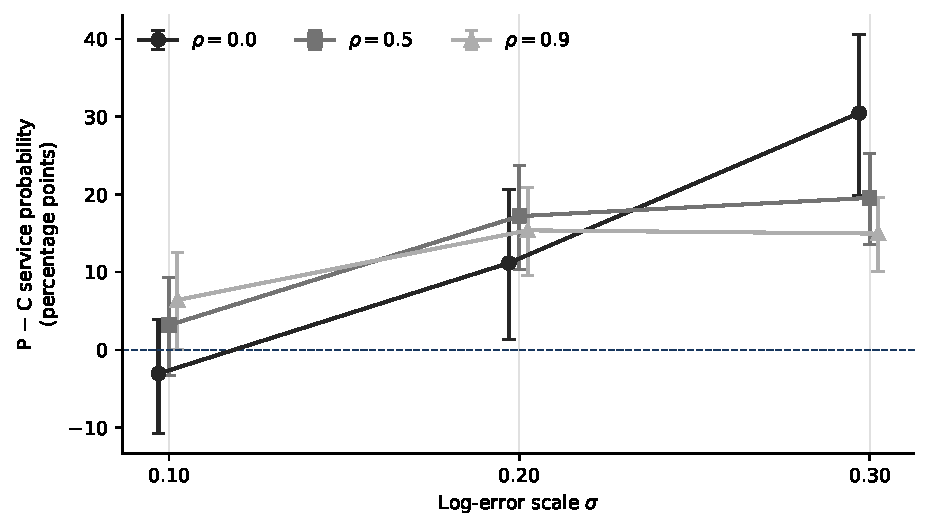
\includegraphics[width=0.93\textwidth]{Fig1.pdf}
 \caption{Paired difference in service probability between the original
 procedure (P) and conservative-speed planning (C) on the 46 common instances.
 Circles, squares and triangles mark $\rho=0$, $0.5$ and $0.9$, and the dashed
 line marks zero. Faint vertical lines mark $\sigma=0.10$, $0.20$ and $0.30$;
 markers are offset slightly around them only for legibility. Error bars are
 95\% bootstrap intervals over instances. Plans are fixed across this
 disturbance sweep, and the intervals are not simultaneous across cells.}
 \label{fig:reliability}
\end{figure}

\input{confirmatory_results.tex}
\input{weight_results.tex}
\input{weight_bracketing.tex}
\input{solomon_results.tex}
\input{study2_results.tex}
\input{gh_results.tex}
\input{robust_results.tex}
\input{robust_extra.tex}
\input{fallback_results.tex}
\input{checks_summary.tex}

Section~\ref{sec:additional} reports the results of the first two confirmatory studies by
size (Tables~\ref{tab:conf-size} and~\ref{tab:study2-size}, descriptive only), every robust setting
(Table~\ref{tab:robust-grid}), customer outcomes on the matched
subset (Table~\ref{tab:customers}), absolute planned resources
(Table~\ref{tab:fullcost}), service-threshold sensitivity
(Table~\ref{tab:kappa}), the instance-level failure audit
(Table~\ref{tab:failure}), and the equal-budget deterministic benchmark against
PyVRP/HGS (Table~\ref{tab:hgs}).

\section{Reproducibility and implementation checks}\label{sec:reproducibility}

The study archive \cite{ali2026archive} contains the candidate generators, the
scenario-bank code, the test suite, the experiment drivers, the raw JSON records
and the scripts that produce the results tables and the figures. The tests cover
FIFO behaviour, lognormal moments, common random numbers that do not depend on
evaluation order, Wilson calculations, visit and capacity feasibility, the rule
that contracted candidates are scored against the original windows, and the
robust feasibility checks, which are compared with brute-force enumeration of
deviation sets. Each run
records the Python, NumPy and OR-Tools versions, the operating system, the solver
budget, the seeds and the scenario counts.

The clock convention matters for reproduction. Relative time zero is 06:00, and
the evaluator adds 360 minutes before looking up the full-day speed profile;
leaving out that offset would evaluate a 00:00--10:00 shift instead. The
vectorized evaluator is checked against the original scalar implementation,
including period boundaries, customer lateness and shared arc disturbances.

Seeds are fixed. Admission uses seed $100000$ plus the instance seed, all
validation uses 5000 fresh scenarios from seed $400000$ plus the instance seed,
and the 1000-scenario disturbance sweep uses seed $500000$ plus the instance
seed. The capped, screened-conservative and clock-aware configurations were specified
before they were run on the development instances, but earlier aggregate results
motivated them, so they are exploratory and are neither preregistered nor an
external replication; the fresh scenario draws do not
remove the reuse of the instance set. Plans in the sweep are not re-screened when
$\sigma$ or $\rho$ changes.

The first confirmatory protocol (Section~\ref{sec:confdesign}) was publicly
timestamped, with a hash manifest of the code that runs and analyses it, before
its instances were solved; its results are in Section~\ref{sec:confirmatory}. One
pipeline smoke test, on an instance outside the confirmatory set, was run while
the protocol was being prepared, and the protocol discloses it as pilot data. The
confirmatory study used only frozen scripts. The weight-sensitivity analysis was
run after the freeze with a script outside the frozen file list. Its first run
stopped on a coding error that affected only that script, and the corrected
script produced the reported results. The second confirmatory study
(Section~\ref{sec:conf2design}) has its own frozen protocol and manifest. Its
OR-Tools half uses the frozen scripts of the first study, and its HGS half is
deterministic given the scaling ranges. The script that writes its tables and
text stops unless its verdicts and counts equal the saved output of the frozen
analysis and its estimates agree with that output to its two-decimal rounding.
The one-decimal figures in the paper are rounded from the exact estimates, and
those of the first study are produced in the same way. The development robust comparison (Section~\ref{sec:robust-design}) was run after
both studies with code outside the frozen file lists. Its search stops after a
fixed number of iterations with a fixed seed, so its plans are deterministic, and
the script that writes its tables and figure checks that every record is present
and complete. The third protocol (Section~\ref{sec:conf3design}) and its manifest
were committed publicly and archived \cite{ali2026freeze3} before any of its
runs; part B started one minute after the release. Its OR-Tools half was
interrupted once by a restart of the machine; the frozen drivers resume from the
records already written, so completed instances were kept and the remaining ones
were run afterwards. Both analysis programs ran once in confirmatory mode, after
all records were complete.

All results tables and both figures are regenerated from the retained records. Internal
planning buffers are always evaluated against the offered windows, candidate
selection and final assessment use independent banks, and solver-quality
comparisons between OR-Tools and HGS use equal wall-clock budgets on identical
deterministic instances. These rules stop diagnostics and within-run selection
from using their own validation outcomes. The robust search is compared with HGS
at fixed iteration counts. The family-wise, timing and misspecification checks
(Section~\ref{sec:checks}), the post hoc fallback comparison, the fleet-matched
robust contrast, the weight bracketing and the Gehring--Homberger check also use
code outside the frozen lists. The family-wise script first repeats every stored selection with
the original bound and stops unless all of them match, and the evaluator for the
alternative delay models reproduces the stored validation results exactly when
given the paper's model and validation seeds. A test checks this on OR-Tools,
HGS and robust plans of every instance size.

Reproducibility shows that the reported numbers follow from the archived code and
records. It does not show that the synthetic instances or the assumed disturbance
model represent a real operation.


\clearpage
\section{Origin of the weight vector}\label{sec:ahp-matrix}

The baseline weights were first computed from an Analytic Hierarchy Process
matrix. They are used in this paper as a fixed experimental vector, and this
appendix records their origin only. Criteria are ordered as distance cost, slack deficit, driver duration and fleet
use. Entry $a_{kl}$ is the judged importance of criterion $k$ relative to $l$
on Saaty's 1--9 scale:
\[
\mathbf{A}=\begin{pmatrix}
1 & 3 & 5 & 7\\
1/3 & 1 & 3 & 5\\
1/5 & 1/3 & 1 & 2\\
1/7 & 1/5 & 1/2 & 1
\end{pmatrix}.
\]
Its principal eigenvalue is $\lambda_{\max}=4.0685$, and the normalised
principal eigenvector is
\[
\mathbf{w}=(0.5693,\;0.2643,\;0.1055,\;0.0609).
\]
With Saaty's random index 0.90 for four criteria, the consistency index is
$(4.0685-4)/3=0.0228$ and the consistency ratio is $0.0254$. As stated in Section~\ref{sec:objective-scaling},
the third row and column were set when the third criterion was total distance
and were not re-elicited for driver duration.

\section{Additional outcomes and failure records}\label{sec:additional}
\input{confirmatory_appendix.tex}
\input{study2_appendix.tex}
\input{robust_appendix.tex}
\input{additional_results_v7.tex}
\clearpage
\input{checks_results.tex}
\clearpage


\clearpage
\bibliographystyle{itor}
\bibliography{itor_refs}
\end{document}
